\section{Objektorientierung}

Objektorientierung soll es erleichtern, eine Abbildung der Realität zu erstellen. 
Viele Dinge aus der Wirklichkeit können als Modell dargestellt / simplifiziert werden. 
Diese Modelle können in Software in sogenannte Objekte \texttt{umgewandelt} werden.

\subsection{Objekte}

Objekte stellen Dinge, Sachverhalte oder Prozesse dar. Sie sind ein rein gedankliches Konzept.\\
Sie kennzeichnen sich durch:

\begin{itemize}[itemsep=1pt, parsep=0pt]
    \item eine \textbf{Identität}, welche es erlaubt Objekte voneinander zu unterscheiden
    \item \textbf{statische Eigenschaften} zur Darstellung des \textbf{Zustandes} des Objekts in Form von \textbf{Attributen}
    \item \textbf{dynamische Eigenschaften} zur Darstellung des \textbf{Verhaltens} des Objekts in Form von \textbf{Methoden}
\end{itemize}


\subsection{Klassen \& Instanzen}

Ähnliche Objekte können in \textbf{Klassen} zusammengefasst werden, um Programmieraufwand tiefer zu halten. 
Verwendete Objekte werden als \textbf{Instanz} eingesetzt. Diese Objekte haben dieselben Attribute, allerdings andere Werte.\\
Eine Beispielklasse:

\lstinputlisting{code/03_Objektorientierung/class_example.cpp}\vspace{-1em}

\subsubsection{Reihenfolge der Header-Datei (.h)}

\begin{enumerate}[itemsep=1pt, parsep=0pt]
    \item Dateikommentar mit Lizenzvereinbarung.
    \item \textit{\color{blue} \texttt{Includes} des verwendete System Header \texttt{<\dots>}}
    \item \textit{\color{blue} \texttt{Includes} der Projektbezogenen Header \texttt{"\dots"}}
    \item \textit{\color{blue} Definition von Konstanten}
    \item \textit{\color{blue} Typedef's und Definitionen von Strukturen}
    \item \textit{\color{blue} allenfalls extern-Deklaration von Global-Variablen}
    \item \textit{\color{blue} Funktionsprototypen, ink. Kommentar der Schnittstelle, bzw. Klassendeklarationen}
\end{enumerate}

\begin{itemize}
    \item Die \textit{blauen} Punkte müssen sich im Includeguard befinden(\#pragma once).
    \item Pro Header-Datei sollte nur eine Oberklasse deklariert sein. 
    \item Kleine Unterklassen können im gleichen Header stehen.
    \item Kein \lstinline[language=C++]|using namespace ...| in header files
\end{itemize}

\subsubsection{Reihenfolge der Implementation (.cpp)}

\begin{enumerate}[itemsep=1pt, parsep=0pt]
    \item Dateikommentar mit Lizenzvereinbarung
    \item \texttt{includes} der eigenen Header
    \item \texttt{includes} der Projektbezogenen Header
    \item \texttt{includes} der verwendeten System Header
    \item allenfalls globale und statische Variablen
    \item Präprozessor-Direktiven
    \item Funktionsprototypen von lokalen, internen Funktionen (in nameless Namespace)
    \item Definition von Funktionen und Klassen (\crd{Kommentare nicht wiederholen})
\end{enumerate}

\subsection{UML}

Die \texttt{Unified Modeling Language} ist eine normierte Sprache um Objekte grafisch 
darzustellen, \textbf{programmierspracheunabhängig}.

\subsubsection{UML-Klassendiagramm Notation}

Besteht immer aus 3 Boxen:\vspace{1em}

\noindent
\begin{minipage}{0.4\columnwidth}
\begin{center}
        \begin{tikzpicture}
        \node [umlclass] (Student) { % siehe Präambel umclass style
            \centering \textbf{Student}
            \nodepart{second}
                + IDNumber : int \\
                \# name : string \\
                - bierkonsum : float \\
                \# investedTimeInET : int
            \nodepart{third}
                - doStuff(time : int) \\
                + \textit{useless()}
        };
    \end{tikzpicture}
\end{center}
\end{minipage}
\begin{minipage}{0.57\columnwidth}
    \begin{itemize}
        \raggedright
        \item Zu oberst der Name 
        \item In der Mitte Attribute(Variablen)
        \item Unten Methoden.
        \item Methoden und Attribute fangen mit einem Symbol an, welches die \textbf{Sichtbarkeit} 
                definiert und haben ein bestimmtes Merkmal:
        \item Wörter wie \lstinline[language=C++]|void| o. \lstinline[language=C++]|const| sind sprachspezifisch, nicht einfügen
    \end{itemize}
\end{minipage}\vspace{1em}

\begin{itemize}[itemsep=1pt, parsep=0pt]
    \item + : public (überall sichtbar)
    \item - : private (nur in  aktueller Klasse sichtbar)
    \item \# : protected (in aktueller und Unterklassen sichtbar)
    \item \textit{Italic} : Funktion oder Klasse ist Abstrakt (=0)
    \item \underline{Unterstrichen} : Funktion oder Attribut ist static
    \item \verb|<Name der Klasse>| :  Konstruktor (ohne \verb|<>|)
    \item $\sim$\verb|<Name der Klasse>| : Destruktor (ohne \verb|<>|)
\end{itemize}



\subsection{class vs struct}

Eine class und struct können fast identisch verwendet werden. 
Eine class hat \textbf{standardmässig Sichtbarkeit private} sonst muss explizit mit \lstinline[language=C++]|public:| gekennzeichnet, Struct public(wenn nichts definiert wird).

\subsubsection{Zugriffsschutz}
\begin{tabular}{|l|l|}
    \hline
    \textbf{Modifikator} & \textbf{Beschreibung \& Best Practice} \\ \hline
    \lstinline[language=C++]|public| & Zugriff von innerhalb und von ausserhalb der Klasse. \\ 
    & $\rightarrow$ Fast alle \textbf{Methoden} sind public. \\ 
    & $\rightarrow$ \textbf{Attribute} sollten \textit{nie} public sein. \\ \hline
    \lstinline[language=C++]|protected| & Zugriff von innerhalb der Klasse und den \textbf{abgeleiteten Klassen}. \\ 
    & $\rightarrow$ Nur sehr sparsam zu verwenden. \\ \hline
    \lstinline[language=C++]|private| & Zugriff \textbf{nur} von innerhalb der eigenen Klasse aus. \\ 
    & $\rightarrow$ Für alle Attribute und für spezifische lokale Methoden. \\ \hline
\end{tabular}

\subsection{Inkludierte Dokumentation}

Mann kann im H-File direkt die Dokumentation zu der Schnittstelle schreiben. 
Das ermöglicht das einfachere Verwenden der Schnittstelle.

\lstinputlisting{code/03_Objektorientierung/codedocumentation.cpp}

Es kann immer mehr geschrieben werden, man sollte sich aber auf das Nötige beschränken.

\section{Konstruktoren und Destruktoren}

Konstruktoren (CTOR) und Destruktoren (DTOR) sind spezielle Methoden, die den Lebenszyklus des Objekts steuern. 
Beide haben den exakten Klassennamen und haben \textbf{keinen} Rückgabetyp (nicht einmal \lstinline[language=C++]|void|).

\subsection{Konstruktoren (CTOR)}

Hauptaufgabe des CTORs ist die "saubere" Initialisierung aller Attribute der Klasse.

\begin{itemize}
    \item \textbf{Default-Konstruktor:} Hat keine Parameter. Wird automatisch aufgerufen, wenn das Objekt ohne Argumente deklariert wird (z.B. \lstinline[language=C++]|Stack s;|). 
    Falls nicht definiert, erstellt der Compiler einen implizit (der aber primitive Typen nicht initialisiert).
    \item \textbf{Copy-Konstruktor:} Erhält eine \lstinline[language=C++]|const|-Referenz auf eigene Klasse (\lstinline[language=C++]|TString(const TString& s)|). 
    Wird benutzt, um ein Objekt als Kopie eines bestehenden zu erzeugen.
    \item \textbf{Explicit-Konstruktor:} Markiert man einen CTOR mit 1 Parameter als \lstinline[language=C++]|explicit|, verhindert man ungewollte implizite Konversionen (es. \lstinline[language=C++]|TString s = 5;|).
\end{itemize}

Werden verschiedene Konstruktoren definiert, muss der Default zuerst aufgerufen werden, wenn dieser erhalten bleiben soll.

\subsubsection{Best Practices di Inizializzazione}
Eine Hauptverantwortung des Konstruktors ist es, zu garantieren, dass das Objekt in einem validen Zustand entsteht. 
Das heisst, dass \textbf{alle} Klassen-Attribute auf einen definierten Wert initialisiert werden müssen.

\begin{itemize}
    \item \textbf{Assegnamento nel corpo (\ref{chap:ctor_dtor_example}):} Weniger effizient, Member werden erst mit Default-Werten erzeugt und danach überschrieben.
    \item \textbf{Initialisierungsliste (\ref{chap:user_ctor}):} Die bevorzugte Methode aus Effizienzgründen; Attribute werden direkt bei der Erstellung initialisiert.
    \item \textbf{Member In-Class Initialization:} (Ab C++11) Erlaubt Default-Werte direkt in der Klassendeklaration zu setzen, was CTORs vereinfacht und Vergessen verhindert.
\end{itemize}

\subsection{Gestione Memoria: Shallow vs. Deep Copy}

Wenn eine Klasse Pointer auf dem Heap allokierten Speicher (\lstinline[language=C++]|new|) verwaltet, ist das Default-Verhalten kritisch:

\begin{description}
    \item[Shallow Copy (Default):] Der Compiler kopiert lediglich die Adresse des Pointers. 
    Beide Objekte zeigen auf denselben Speicher. Gibt einer ihn frei, zeigt der andere auf ungültigen Speicher (\textit{Double Free} oder \textit{Segmentation Fault}).
    \item[Deep Copy (Manuale):] \textbf{\color{red}Zwingend nötig} ist ein eigener Copy-Konstruktor, der neuen Platz auf dem Heap allokiert und die Nutzdaten kopiert.
\end{description}

\subsection{Destruktor}

Ein Destruktor eintfernt eine Instanz aus dem Speicher, 
hat keine Aufrufparameter und auch kein Rückgabewert.
Es kann immer nur \textbf{einen} Destruktor geben. 
Wenn der Destruktor fertig ist, sollte kein Speicher mehr vom Objekt belegt sein.\\
Destruktoren sollten immer \textbf{virtuell definiert werden} (siehe \ref{Virtual}). 
Mit anderen virtuellen Funktionen \textbf{müssen} sie virtuel definiert werden. 
Der Funktionsname beginnt mit einer Tilde($\sim$). 
Der Destruktor wird evtl. auch Implizit aufgerufen z.b., wenn aus einer Funktion wieder herausgesprungen wird.

\subsection{Beispiel}\label{chap:ctor_dtor_example}

\lstinputlisting{code/03_Objektorientierung/constructor.cpp}

\section{Initialisierungslisten und direkte Initialisierung}

Die Initialisierung von Datentypen kann auf verschiedene Arten erreicht werden. 
Es wird zwischen Zuweisung und Initialisierung unterschieden.

\subsection{POD's}

\texttt{plain old datastructure} / built in datatypes

\lstinputlisting{code/03_Objektorientierung/pod_init.cpp}

\subsection{Non PODs}

\lstinputlisting{code/03_Objektorientierung/non_pod_init.cpp}

\subsection{User defined Constructor}\label{chap:user_ctor}

Um eine Klasse richtig initialisieren zu können muss der Ctor korrekt definiert werden.
Eine sogenannte \textbf{Initialisierungsliste} wird verwendet:

\lstinputlisting{code/03_Objektorientierung/userdefined_ctro.cpp}

\section{Assertions}
Assertions sollten Annahmen über korrekte Wertebelegung darstellen.
Sie sind kein C spezifisches Konzept und sollten \textbf{nur zu Testzwecken} eingesetzt werden. 
Im Releasebuild sollten sie deaktiviert werden. Dafür gibt es spezifische Präprozessorflags.
Der Header \textbf{$<$assert.h$>$} bzw. \textbf{$<$cassert$>$} stellt hierfür ein Präprozessor-Makro \lstinline[language=C++]|assert(Bedingung)|
zur Verfügung, um solche Zusicherungen auszudrücken.\\
\textbf{Beispiel}:

\lstinputlisting{code/03_Objektorientierung/assertions.cpp}

Das obige Beispiel hat eine Assertion. 
Diese würde im Test, falls ein Nullpointer übergeben wird ein Fehler ausgegeben.

\section{This-Pointer}

Mit dem \texttt{this Pointer} kann ein Pointer des aufrufenden Objekt zurückgegeben werden.
Bsp:

\lstinputlisting{code/03_Objektorientierung/this_pointer.cpp}

Nacheinander werden diese Funktionen durchlaufen da Funktion(2) vom zurückgegebenen Pointer aus Funktionsaufruf 1 aus gerufen wird.
Die funktion wird \textbf{Kaskadiert}


\section{Overloading}

Operator Overloading bedeutet das bestehende Operatoren \texttt{überladen} werden im Sinne neu definiert / darüber geladen.
Sie erhalten \textbf{neue Bedeutung} für eine Klasse.


\subsection{Methodenoverloading}
\begin{itemize}
    \item \textbf{Definition}: Gleicher Name für Funktionen mit anderen Parametern (Typ, Anzahl, Reihenfolge).
    \item \textbf{Signatur}: Besteht aus \textit{Name + Paramtern}. Der Rückgabetyp ist \textbf{exkludiert}.
    \item \textbf{Regel}: Unterscheiden sie sich nur im Rückgabetyp, generiert der Compiler einen Error.
    \item \textbf{Best Practice}: Overloading nur für vergleichbare Ops nutzen und \textbf{nie mit Default-Parametern vermischen.}
\end{itemize}

\begin{center}
    
    \begin{tabular}{lll}
        \toprule
        \textbf{Eigenschaft} & \textbf{Overloading} & \textbf{Default Parameter} \\
        \midrule
        Speicher & Mehr Funktionen & Eine Funtkion \\
        Wartung & Höher & Geringer \\
        Flexibilität & Verschied. Typen & Vordefinierte Werte \\
  
        \bottomrule
    \end{tabular}
\end{center}

\lstinputlisting[language=c++]{code/03_Objektorientierung/method_overloading.cpp}

\subsection{Operator overloading}

Es können die inkludierten Operatoren von C++ überladen werden.

% \begin{itemize}
%     \item Die Anzahl an Operanden und die Bindungsrichtung (links nach rechts) kann \textbf{nicht} verändert werden.
%     \item Die Präzedenz (Vorrangregeln) kann \textbf{nicht} verändert werden.
%     \item Es können \textbf{keine} neuen Operatoren erfunden werden.
% \end{itemize}

Erlaubte Operatoren sind:\\
\begin{tabular}{lllllllll}
    +            & -               & * & ⁄                      & \%                           & $\wedge$ 
                & \&                            & $|$              & $\sim$          \\
    !
& =               & \textless{} & \textgreater{}         & +=                           & -=                      & *=                    
        & ⁄=               & \%=             \\
    $\wedge$=    & \&=             & $|$=        & \textless{}\textless{} & \textgreater{}\textgreater{} & \textless{}\textless{}= & \textgreater{}\textgreater{}= & ==               & !=      
        \\
    \textless{}= & \textgreater{}= & \&\&        & $\|$                   & ++                           & $--$                    & ,      
                       & -\textgreater{}* & -\textgreater{} \\
    ( )          & {[} {]}         & new         & delete                 & new{[} {]}                 
  & delete{[} {]}           &                               &                  &                
\end{tabular}\medskip

Nicht erlaubte Operatoren sind: '\lstinline[language=C++]|.|
\quad \lstinline[language=C++]|.*| \quad \lstinline[language=C++]|::| \quad \lstinline[language=C++]|?:| \quad \lstinline[language=C++]|sizeof| \quad \lstinline[language=C++]|typeid|'.
Es wird zwischen Overloading als \textit{globalen Funktion} und als \textit{Klassen-Methode} unterschieden.

\subsubsection{Als Methode (Member function)}

Ein Operator kann als Methode einer Klasse definiert werden. 
Dies ist der Standardfall, wenn der \textbf{linke Operand} ein Objekt der eigenen Klasse ist.
Der linke Operand (Objekt selbst) ist dabei implizit, weshalb die Methode \textbf{einen Parameter weniger} annimmt als die globale Variante.\\
Syntax: \lstinline[language=C++]|<returntype> operator<typ>(type in);|
\begin{itemize}
    \item \textbf{Visibilità a livello di Classe:} In C++ agiert die Zugriffskontrolle (\lstinline[language=C++]|private|) auf Stufe der \textbf{Klasse}, nicht des einzelnen Objekts.
    \item \textbf{Accesso Incrociato:} \cor{Eine Methode der Klasse $A$ darf auf private Member \textit{jeglicher} Instanz des Typs $A$ zugreifen.}
    \item \textbf{Applicazioni:} Diese Eigenschaft ist unverzichtbar um Operator Overloading (z.B. \lstinline[language=C++]|operator+|), Copy-Konstruktoren oder Vergleichsmethoden zu bauen, wo ein Objekt interne Daten seines "Gleichen" lesen muss.
\end{itemize}

\lstinputlisting{code/03_Objektorientierung/operator_overloading_method.cpp}

\textbf{Zwingend als Elementfunktion zu implementieren}
\begin{itemize}
    \item Zuweisung (\lstinline[language=C++]|=|, \lstinline[language=C++]|+=|, etc.)
    \item Index \lstinline[language=C++]|[]|
    \item Funktionsaufruf \lstinline[language=C++]|()|
    \item Zeigeroperator \lstinline[language=C++]|->|
\end{itemize}

\subsubsection{Als globale Funktion (Global)}

Globales Overloading wird \textbf{zwingend benötigt}, wenn der \cor{\textbf{linke Operand} \textit{nicht} 
von der eigenen Klasse ist.} Typische Beispiele sind:
\begin{itemize}
    \item Ein primitiver Datentyp links (z.B. \verb|string + TString|).
    \item I/O Stream-Operatoren wie \textless{}\textless{}, bei denen der linke Operand ein Stream-Objekt ist (z.B. \verb|std::cout << obj|).
\end{itemize}

Syntax: \verb|<returntype> operator<type>(type val1, type val2);|\medskip

\textbf{Friend Keyword:}\\
Oft müssen globale Operatorfunktionen auf private Daten der Klasse zugreifen. 
In diesem 
Fall werden sie innerhalb der Klasse mit dem Keyword \lstinline[language=C++]|friend| deklariert. 
Dadurch erhalten sie als globale Funktionen Zugriff auf \textbf{alle privaten Attribute 
und Methoden} der Klasse, ohne selbst Teil der Klasse (Methode) zu sein. 
\crd{\textit{Achtung}: Friend-Funktionen sollten gezielt eingesetzt werden.}

\lstinputlisting{code/03_Objektorientierung/operator_overloading_global.cpp}

\textbf{Beispiel I/O Streams (\lstinline[language=C++]|<<|):}\\
Damit Verkettungen wie \verb|cout << a << b;| 
funktionieren, muss als Rückgabewert eine Referenz auf den \verb|ostream| geliefert werden (\verb|return os;|).
\lstinputlisting[language=C++]{code/03_Objektorientierung/03_Objektorientierung_snippet_1.cpp}

\subsubsection{Operatoren und Typumwandlungen}
\begin{itemize}
    \item Um unzählige Varianten eines Operators für jede Typkombination zu vermeiden, kann man \textbf{benutzerdefinierte Typumwandlungen} nutzen.
    \item Ein einzelner Operator kann diverse Inputs handhaben, falls ein Konstruktor existiert, der diese Typen in die Zielklasse wandelt.
\end{itemize}

\lstinputlisting[language=C++]{code/03_Objektorientierung/operatoren_typumwandlung.cpp}

\section{Getter \& Settermethoden}

Getter und Settermethoden werden Typischerweise verwendet um Lese und Schreibzugriffe auf eine Klasse zu regeln. 
Attribute sind \textbf{alle Parameter einer Klasse}.
Mit einer Get oder Set Methode kann der Zugriff auf diese kontrolliert / angepasst werden.\medskip

\cor{\lstinline[language=C++]|const| after the funtion name declares that the method cannot modify any Attribute} 

\myul{immer fur Selector (Getter) benutzen}

\lstinputlisting{code/03_Objektorientierung/getter_settermethoden.cpp}

\subsubsection{Mutable}
Gewisse Attribute dürfen von \lstinline[language=C++]|const| Methoden geändert werden mit dem \lstinline[language=C++]|mutable| Keyword, \textbf{so wenig wie möglich nutzen}
\begin{lstlisting}
...
mutable int error;
...
\end{lstlisting}

\subsubsection{Const correctness}
\begin{itemize}
    \item \textbf{Nur Lesen:} Ein als \lstinline[language=C++]|const| deklariertes Objekt darf \textit{nur} \lstinline[language=C++]|const| Methoden aufrufen.
    \item \textbf{Sicherheit:} Ist eine Methode nicht als \lstinline[language=C++]|const| markiert, nimmt der Compiler an, sie ändere das Objekt und verbietet sie auf konstanten Instanzen, um Seiteneffekte zu vermeiden.
\end{itemize}

\example{}
\lstinputlisting[language=C++]{code/03_Objektorientierung/03_Objektorientierung_snippet_2.cpp}

\section{Vererbung}

Vererbung erlaubt es Attribute und Methoden von anderen Klassen zu übernehmen. 
Die Oberklasse, Baisklasse oder Superklasse \texttt{vererbt} an eine Unterklasse, derived class oder eine Spezialisierung. 
Bei der Vererbung werden immer \textbf{alle} Attribute oder Methoden weitergegeben. 
\subsubsection{UML}

In einem UML Diagramm wird vererbung wie folgt dargestellt:\\
\noindent
\begin{minipage}{0.6\columnwidth}
    \input{tikz/uml.tex}
\end{minipage}\hfill
    \begin{minipage}{0.35\columnwidth}
    Unterklasse erbt (die Attribute und Methoden) von Superklasse.
\end{minipage}\vspace{1em}

Dies stellt eine \texttt{ist ein beziehung} dar. 
Es ist sehr wichtig, dass die Pfeilspitze \colorbox{red!65}{\textbf{genau so!}} aussieht wie in der Darstellung da ansonsten Verwechslungsgefahr mit anderen Mechanismen entstehen könnte.
\subsubsection{Syntax}

\lstinputlisting{code/03_Objektorientierung/vererbung_syntax.cpp}

\subsubsection{UML++}

\input{tikz/umlpp.tex}
\hfill
\begin{minipage}[b]{0.45\columnwidth}
    Vererbung ist auch über mehrere Stufen Möglich:\\
    Z.b. C4 Erbt alles von C2 und C1
\end{minipage}

\subsubsection{Sichtbarkeit}

Die Sichtbarkeit ist durch das Public definiert. 
Es ist möglich die Sichtbarkeit aller Attribute und Methoden einzuschränken. 
Mit \textbf{Public} wird alles mit der originalen Sichtbarkeit übernommen. 
Mit \textbf{protected} wird alles was public war protected. 
Mit \textbf{private} wird alles private (nicht sehr nützlich). 
\resizebox{\columnwidth}{!}{  
    \input{tikz/sichtbarkeit.tex}
}

Wird eine Vererbung private durchgeführt, sind keine Attribute oder Methoden mehr sichtbar.
Attribute soll nie \lstinline[language=C++]|protected| sein
\subsubsection{Constructor / Destructor chaining}

\par{Logica dei Costruttori (CTOR)}
\begin{itemize}
    \item \textbf{Prinzip der Verantwortung:} Der Konstruktor einer Klasse initialisiert explizit \textbf{nur seine eigenen Attribute}.
    \item \textbf{Delegation:} Für Basisklassen-Attribute wird der CTOR der Basisklasse selbst aufgerufen (die Basis "kümmert sich um ihre eigenen Dinge").
    \item \textbf{Prioritätsregel:} Die Elemente der Basisklasse müssen \textbf{immer als erstes initialisiert werden}.
\end{itemize}


\lstinputlisting{code/03_Objektorientierung/ctor_unterklasse.cpp}

\par{Logica dei Distruttori (DTOR)}
\begin{itemize}
    \item \textbf{Umgekehrte Reihenfolge:} DTORs werden in der exakt umgekehrten Reihenfolge der CTORs ausgeführt.
    \item \textbf{Ausführungs-Reihenfolge:} Von unten nach oben (Subklasse $\rightarrow$ Basisklasse).
\end{itemize}

\subsection{Überschreiben von Methoden}

Geerbte Funktionen können \texttt{überschrieben} werden. 
Die Unterklasse definiert eine neue Methode mit demselben Namen.
Allerdings kann es dann zu Mehrdeutigkeit kommen:\\
Im folgenden Beispiel haben eine Subklasse und eine Oberklasse eine print Funktion welche \textbf{nicht} virtual gekennzeichnet ist:

\lstinputlisting{code/03_Objektorientierung/methodenueberschreiben.cpp}

Dieses Beispiel soll zeigen, dass Pointer, welche eigentlich von einer Oberklasse auf eine Unterklasse zeigen auf die \texttt{Eigenen} Funktionen der Oberklasse zeigt, solange diese nicht überschrieben worden sind. 
Dies kann als Verhalten gewünscht sein. 

\subsection{virtual, final, override und scopeoperator}

\subsubsection{virtual}\label{Virtual}
\begin{itemize}
    \item \textbf{Zweck:} Kennzeichnet Methoden, die in Unterklassen überschrieben werden sollen. 
Dies ermöglicht \textbf{Dynamic Binding}, sodass zur Laufzeit immer die spezialisierte Methode der Unterklasse aufgerufen wird.
    \item \textbf{Polymorphie:} Eine Klasse, die mindestens eine virtuelle Funktion besitzt, wird als \textbf{polymorph} bezeichnet.
    \item \textbf{Vererbung:} Einmal als \lstinline[language=C++]|virtual| deklariert, bleibt die Methode in der gesamten Vererbungskette virtuell. 
    \item \textbf{Wichtige Syntax-Regel:} Das Schlüsselwort \lstinline[language=C++]|virtual| darf 
    \textbf{nur bei der Deklaration} (im H-File) verwendet werden.
\end{itemize}

\subsubsection{Virtual beim Dtor}

Ist eine Methode als virtual deklariert, so muss der Dtor \textbf{ZWINGEND} auch als virtual deklariert werden.
\subsubsection{Override}

Soll eine Methode eine geerbte Methode ersetzen so muss diese mit \texttt{Override} gekennzeichnet werden. 
Solch eine Methode ist automatisch auch virtual.
Der Compiler kann so überprüfen, ob eine virtual Methode vorhanden ist.
\subsubsection{Final}

Final kann zum einen verbieten, dass eine Methode einer Klasse überschrieben wird
(Logischerweise geht das nur bei virtuellen Methoden). 
Zum anderen kann sie auch das weitere Erben einer Klasse verbieten.
\subsubsection{Scopeoperator}

Per Scopeoperator kann (::) eine Methode aus einer Oberklasse gezielt aufgerufen werden. 
Mit diesem wird garantiert die Funktion welche definiert wird aufgerufen, egal ob diese aufgrund virtual überschrieben wird. 
\lstinputlisting{code/03_Objektorientierung/virtual.cpp}
\subsection{Classi Polimorfe e Binding}

\begin{itemize}
    \item \textbf{Definition:} Eine Klasse ist polymorph, wenn sie mindestens eine \lstinline|virtual| Fkt deklariert.
    \item \textbf{Datentypen:}
    \begin{itemize}
        \item \textbf{Statischer Datentyp:} Der bei der Deklaration definierte Typ (Typ des Pointers oder der Referenz).
        \item \textbf{Dynamischer Datentyp:} Der effektive Typ des Objekts zur Laufzeit (die echte Instanz).
    \end{itemize}
    \item \textbf{Static Binding (Early Binding):} Passiert während der Kompilierung. Standard für nicht-virtuelle Fkt und hat keinen Overhead.
    \item \textbf{Dynamic Binding (Late Binding):} Funktionswahl passiert zur Laufzeit gemäss dynamischem Typ. Geht nur über Pointer o. Referenzen und hat leichten Overhead via V-Table.
\end{itemize}

\subsubsection{Best Practice e Regole}
\begin{itemize}
    \item \textbf{Distruttori:} Müssen in Basisklassen zwingend \lstinline|virtual| sein, um die korrekte Deallokation der Subelemente zu garantieren, speziell wenn über Pointer der Basisklasse verwaltet.
    \item \textbf{Costruttori:} Dürfen niemals als \lstinline|virtual| deklariert werden.
    \item \textbf{Metodi:} Nur \texttt{virtual} deklarieren, falls Überschreiben geplant ist. Nicht-virtuelle Methoden dürfen in Subklassen nicht überschrieben werden.
    \item \textbf{Override:} In Subklassen müssen überschriebene Methoden explizit mit dem Keyword \texttt{override} markiert werden.
\end{itemize}

\subsubsection{RTTI (Run-time Type Information)}

RTTI erlaubt es, den Typ eines Objekts während der Ausführung zu identifizieren. Si utilizza la funzione \lstinline[language=C++]|typeid()| 
inclusa nell'header \lstinline[language=C++]|<typeinfo>|, welche ein Objekt vom Typ \lstinline[language=C++]|std::type_info| zurückgibt. 
\lstinputlisting{code/03_Objektorientierung/RTTI.cpp}

\subsubsection{Implementazione: La V-Table}

Die techn. Implementation von Polymorphismus und RTTI basiert auf der \textbf{V-Table}:
\begin{itemize}
    \item Jede polymorphe Klasse besitzt eine V-Table mit den Pointern auf ihre virtuellen Funktionen.
    \item Jede Instanz der Klasse enthält einen versteckten Pointer (\textbf{V-pointer}), der auf die V-Table der eigenen Klasse zeigt.
    \item Zur Laufzeit nutzt die Instanz den V-pointer, um die Adresse der korrekten Funktion aufzulösen.
\end{itemize}

Enthält ein Basisklassen-Pointer-Array Objekte verschiedener Subklassen, so hat jedes Objekt einen V-pointer, der auf die spezifische V-Table der eigenen Klasse zeigt, was garantiert, dass korrekte überschriebene Versionen der Methoden aufgerufen werden.
\begin{minipage}{0.42\columnwidth}
    \lstinputlisting[label=cpp]{code/03_Objektorientierung/vtable.cpp}
\end{minipage}
\begin{minipage}{0.58\columnwidth}
    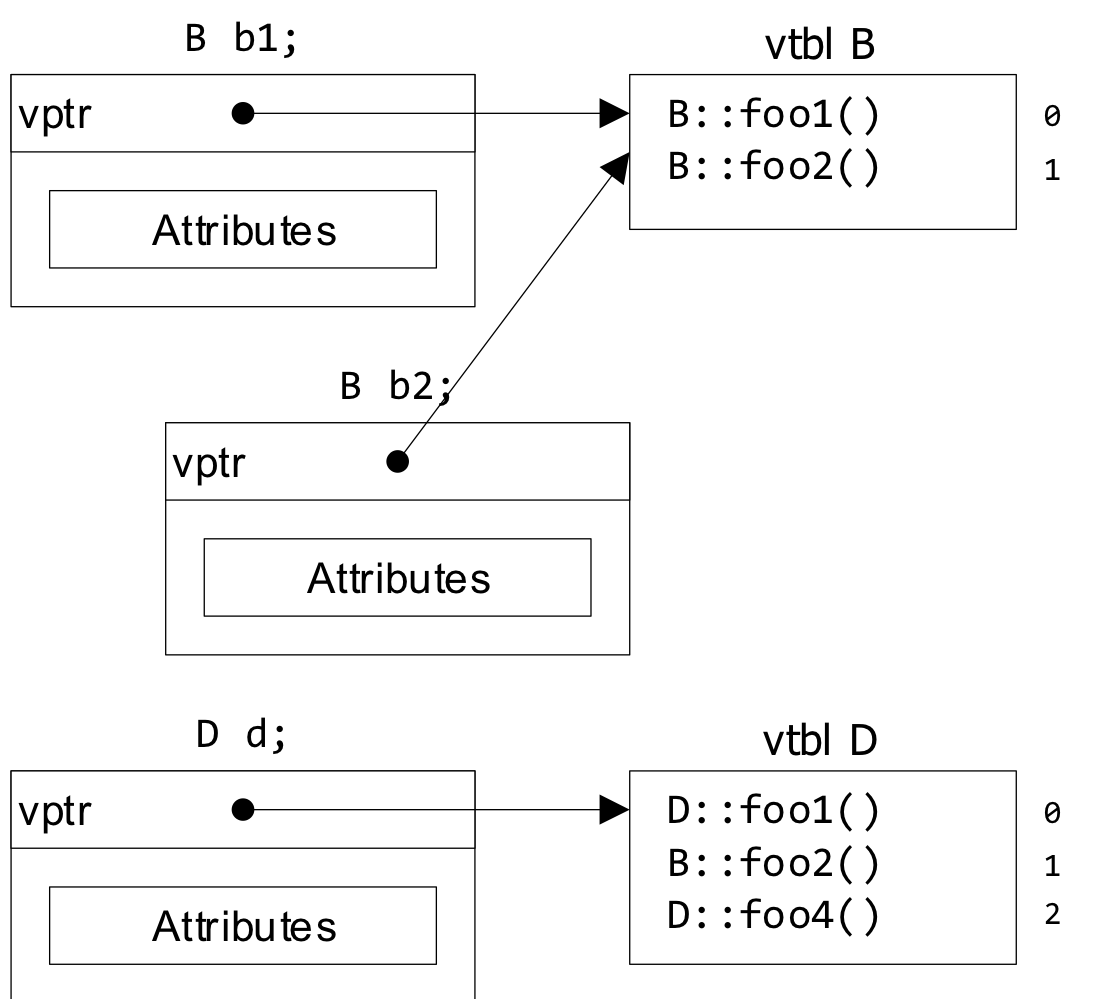
\includegraphics[width=\linewidth]{images/vtable.png}
\end{minipage}



\subsection{Abstrakte Klassen}

Wenn Klassen zwar festlegt, dass eine Methode da ist, diese aber noch nicht implementieren, nennt man das eine abstrakte Methode. 
Man spricht dann von einer abstrakten Klasse.
Eine abstrakte Methode wird in UML \textit{\textbf{kursiv}} dargestellt. 
Es ist egal, ob die abstrakten Methoden selbst definiert sind oder geerbt. 
Abstrakte Klassen kann man nicht instanziieren. 
Es gibt kein spezielles Schlüsselwort dafür, man weist der Methode bei Definition 0 zu: 

\lstinputlisting{code/03_Objektorientierung/abstraktemethode.cpp}

\subsection{Organisation der H files}

Generell gilt immer noch: Jedes H File hat ein Cpp File. 
Allerdings können Unterklassen in ein H File zusammengefasst werden, falls diese nicht allzu Umfänglich sind. 
Ansonsten sollte ein neues H File erstellt werden. 
Für abstrakte Klassen fällt die Implementierung in einem Cpp file weg. 
\subsection{Mehrfachvererbung}

Folgender Vererbungszweig ist möglich:\\
\noindent
\begin{minipage}{0.38\columnwidth}
    \input{tikz/mehrfachverebung.tex}
\end{minipage}
\begin{minipage}{0.62\columnwidth}
Solche Gebilde sind zwar möglich, sollten jedoch vermieden werden, da schnell sehr kompliziert und kaum lesbar. 
Es entsteht schnell Mehrdeutigkeit durch die verschiedenen Erbzweige.\\

Haben 2 Elternklassen eine \cor{\textbf{Methode} mit dem \textbf{gleichen Namen}}, muss sie in der Subklasse neu definiert werden, um das richtige Verhalten festzulegen (ad es. \lstinline[language=C++]|C1::print()|)
\end{minipage}

Bei der Definition einer Klasse können weitere Oberklassen mit einem Komma getrennt angegeben werden
\lstinputlisting{code/03_Objektorientierung/Mehrfachvererbung.cpp}\vspace{-1em}

\subsubsection{Diamond Problem}

\begin{itemize}
    \item \textbf{Das Problem}: Ohne Vorkehrung hätte \texttt{C4} zwei getrennte Kopien von \texttt{C1} (via \texttt{C2} und via \texttt{C3}). \cor{Erzeugt Mehrdeutigkeit beim Member-Zugriff.}
    \item \textbf{Die Lösung (\textit{Virtual Inheritance})}: das Keyword \texttt{virtual} in den mittleren Klassen (\texttt{C2} und \texttt{C3}) weist den Compiler an, eine geteilte Instanz von \texttt{C1} zu bauen.
    \item \textbf{Reihenfolge der Initialisierung}: Folgt einer hierarchischen Priorität:
    \begin{enumerate}
        \item \textbf{Virtuelle Basis}: \texttt{C1} wird als erstes initialisiert.
        \item \textbf{Nicht-Virtuelle Basen}: \texttt{C2} und dann \texttt{C3} (gemäss der Deklarations-Reihenfolge in \texttt{C4}).
        \item \textbf{Abgeleitete Klasse}: Der Body vom Konstruktor von \texttt{C4}.
    \end{enumerate}
\end{itemize}

\lstinputlisting[language=C++]{code/03_Objektorientierung/03_Objektorientierung_snippet_3.cpp}
\subsection{Static} 

Static im Zusammenhang mit Klassen bindet eine Methode oder ein Attribut an die Objektklasse und nicht an die Objektinstanz (ähnlich zu Python Klassenvariablen). 

\subsubsection{Methoden}

Static Methoden müssen im Header-File deklariert und im Cpp-File definiert werden. 
Sie dürfen nur auf Static definierte Attribute zugreifen da \textbf{keine Objektinstanz vorhanden.} 
Hauptanwendungen sind Hilfsfunktionen wie Funktionsaufrufcounter oder Umrechnungsfunktionen. 
Bei der Deklaration wird der Klassennamen verwendet (siehe Bsp). 

\subsubsection{Attribute}

Static Attribute müssen im H deklariert \textbf{und im Cpp File} definiert werden. 
Sie werden verwendet für z.B. Objektspezifische Konstanten oder im Zusammenhang mit Static Counter. 
(\textit{class scope})

\subsubsection{Bsp}

\lstinputlisting{code/03_Objektorientierung/static.cpp}